\documentclass[border=10pt]{standalone}
\usepackage{circuitikz}
\usepackage{tikz}
\usetikzlibrary{calc, positioning, arrows.meta, shapes.geometric}

\begin{document}
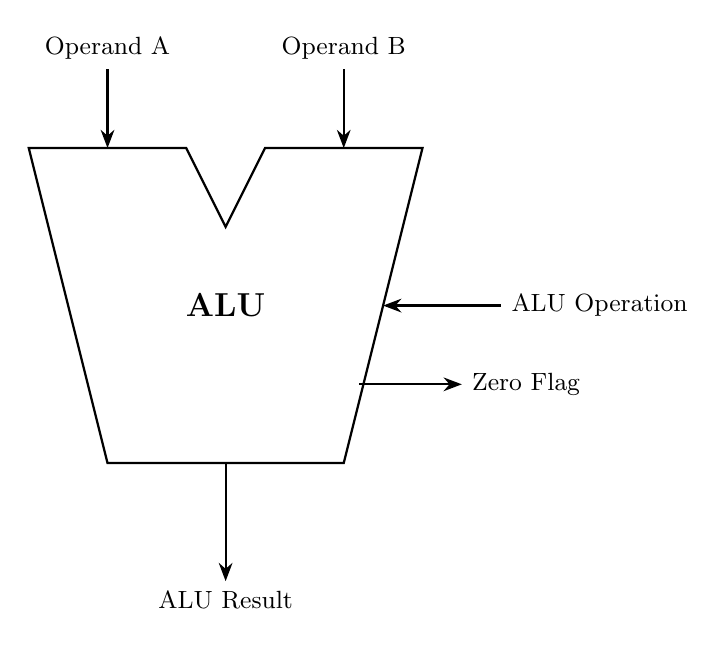
\begin{tikzpicture}[
    >=Stealth, 
    thick, 
    font=\small
]

    % ALU Shape (Manually drawing a trapezoid with V-notch)
    \draw[fill=white] 
        (0, 4) -- (2, 4) -- (2.5, 3) -- (3, 4) -- (5, 4) % Top edge with notch
        -- (4, 0) -- (1, 0) -- cycle;                    % Bottom and sides
    
    \node at (2.5, 2) {\large \textbf{ALU}};

    % Inputs (Top)
    \draw[<-] (1, 4) -- (1, 5) node[above] {Operand A};
    \draw[<-] (4, 4) -- (4, 5) node[above] {Operand B};

    % Control (Side)
    \draw[<-] (4.5, 2) -- (6, 2) node[right] {ALU Operation};

    % Output (Bottom)
    \draw[->] (2.5, 0) -- (2.5, -1.5) node[below] {ALU Result};

    % Flags (Side)
    \draw[->] (4.2, 1) -- (5.5, 1) node[right] {Zero Flag};

\end{tikzpicture}
\end{document}
